\chapter{Een nieuwe UniProtKB-index voor Unipept}\label{ch:een-nieuwe-uniprotkb-index-voor-unipept}
In de vorige hoofdstukken hebben we suffixbomen, suffix arrays, FM-indices en R-indices verkend als indexstructuren die toegepast kunnen worden om een eiwitdatabank te indexeren.
Uit die hoofdstukken bleek namelijk dat een suffix array de laagste geheugenvereisten heeft.
In dit hoofdstuk gaan we dieper in op het opbouwen van een index voor UniProtKB, en het in productie brengen ervan.
Aangezien we de huidige Unipept index willen vervangen door deze nieuwe indexstructuur behandelen we bovendien ook nog enkele extra gewenste features.

\section{Opbouwen van de SA}\label{sec:opbouwen-van-de-sa}
Zoals eerder vermeld levert een ruwe extrapolatie op dat we $\pm$ 1.2 TB aan geheugen nodig zou hebben om een index voor UniProtKB op te bouwen.
Hierbij werd er echter van uitgegaan dat UniProtKB 500\times meer eiwitten dan Swiss-Prot bevat.
Dit is een overschatting van de realiteit waar UniProt op dit moment \textit{slechts} $\pm$ 440 keer groter is.
Dit zorgt ervoor dat het opbouwen mogelijks al \textbf{haalbaar is op HPC van UGent} waar nodes beschikbaar zijn die ongeveer 940 GB aan beschikbaar geheugen hebben.
Na dit te proberen bleek \textit{slechts} 740 GB RAM nodig.
Figuur~\ref{fig:build_uniprot} toont de nodige tijd en hoeveelheid geheugen om dit te realiseren.
\textbf{Opvallend hierbij is dat de libsais implementatie hier trager is dan libdivsufsort}, terwijl dit voor alle kleinere datasets net omgekeerd was.
Afhankelijk van de dataset is het ene algoritme dus sneller dan het andere.
Het geheugengebruik van beide algoritmen blijft echter erg gelijkaardig, wat het belangrijkste is voor ons.
\\
\begin{figure}[H]
    \centering
    \subfloat[Tijd nodig om een SA-index voor UniProtKB te bouwen.]{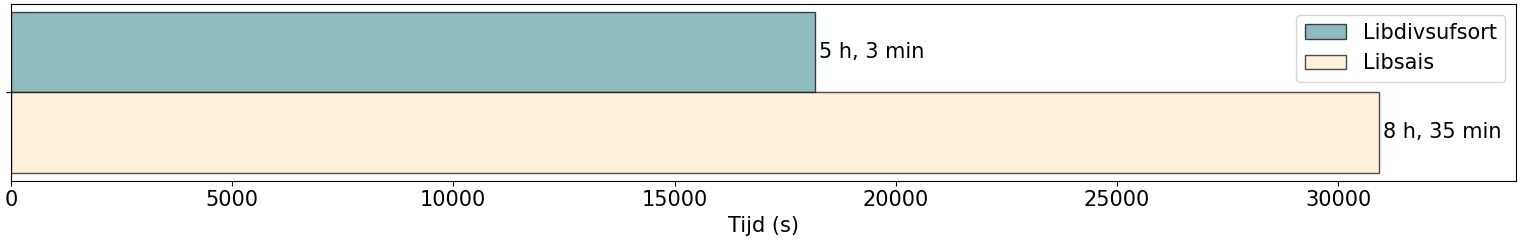
\includegraphics[width=\linewidth]{build_uniprot_time}}\\[4ex] % [4ex] om wat extra vertical spacing in te voegen

    \subfloat[Maximale hoeveelheid geheugen gebruikt tijdens het opbouwen van een SA-index voor UniProtKB.]{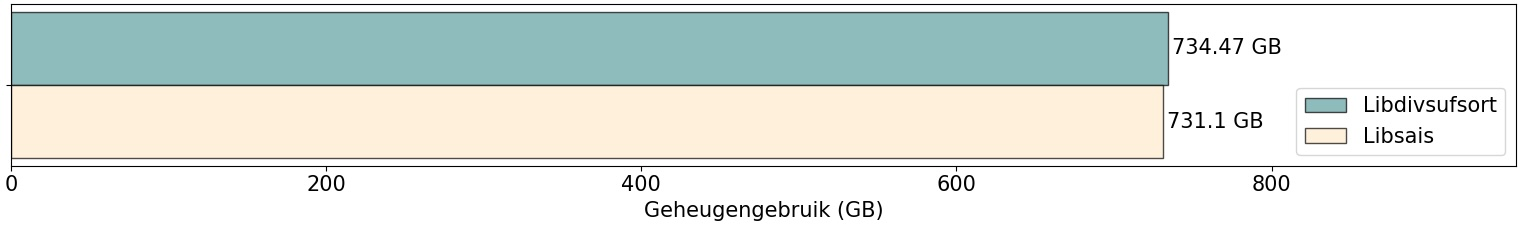
\includegraphics[width=\linewidth]{build_uniprot_memory}}
    \caption{Statistieken voor het opbouwen van een SA voor UniProtKB}\label{fig:build_uniprot}
\end{figure}

\section{Een sparseness factor kiezen}
Een volgende stap na het opbouwen van de volledige SA was het beslissen van de sparseness factor.
Zoals eerder aangegeven in de conclusie van sectie~\ref{subsec:zoeken-in-sparse-suffix-arrays} willen we deze sparseness factor zo laag mogelijk kiezen, met als restrictie dat de SSA nog steeds in het geheugen moet kunnen gehouden worden.
De beschikbare machines die UniPept hosten hebben elk $pm$ 0.5 TB RAM ter beschikking.
Dit wil zeggen dat we de resulterende index hierin moeten krijgen, en ook nog genoeg overhead moeten laten zodat de machine zeker niet out-of-memory gaat tijdens het hosten van de index en het verwerken van meerdere requests.
Praktisch gezien komt dit er op neer dat we gebruikmaken van \textbf{sparseness factor 3}.
Dit resulteert in een SA van 231.81 GB\@.
In combinatie met de tekst (86.93 GB) resulteert dit in een \textbf{totale indexgrootte van 318.74 GB}, wat comfortabel in de 0.5 TB past.
Hierbij moet natuurlijk nog wat overhead gerekend worden om de mapping van de suffix naar proteïne bij te houden.
Bovendien bevatten deze servers ook nog andere databanken om verdere aggregaties te berekenen.
Zo biedt Unipept naast een taxonomische analyse ook nog een functionele analyse aan.
Deze functionele analyse wordt uitgevoerd op basis van de gematchte eiwitten die de indexstructuur terug geeft.
Indien we sparseness factor 2 zouden gebruiken komt de totale indexgrootte uit op $\pm$ 450 GB\@.
Dit op zich zou nog net in de machine passen, maar laat niet genoeg ruimte voor de andere processen.

\section{Isoleucine en Leucine gelijkstellen}\label{sec:isoleucine-en-leucine-equivalentie}
Naast het vinden van exacte matches is het vinden van inexacte matches ook interessant.
Vooral het vinden van matches waarbij we een I (Isoleucine) en L (Leucine) aan elkaar gelijkstellen is een belangrijke optie in de huidige Unipept index.
\textbf{Deze twee aminozuren kunnen niet uit elkaar gehaald worden door een massaspectrometer vanwege hun identieke massa}.
Door deze restrictie van de huidige hardware is het voor onderzoekers erg nuttig om alle matches te vinden waar een I ook een L kan zijn of omgekeerd.
Om deze vorm van inexacte matching toe te voegen aan de index gebruikmakende van een suffix array zijn meerdere opties.
\begin{enumerate}
    \item \textbf{Twee indices:} Bouw een extra index waarbij in de tekst elke L ook door een I vervangen wordt.
    Afhankelijk van als de gebruiker I gelijk wil stellen aan L, wordt daarna de request afgehandeld door de correcte index.
    Hierbij moeten we enkel dezelfde vervangoperatie uitvoeren als bij de index indien I gelijk gesteld wordt aan L\@.
    Deze optie wordt niet verder uitgewerkt omdat we niet alleen twee indices zouden moeten opbouwen, ook de nodige hoeveelheid geheugen om de index te hosten zou verdubbelen.
    Dit is iets wat we willen vermijden.
    \item \textbf{Index waarbij I $\neq$ L:} Genereer de varianten van de gezochte peptide \textit{on the fly} tijdens het zoekproces.
    Hierbij kan gebruikgemaakt worden van het feit dat 2 peptiden die identiek zijn, behalve dat hun I's en L'en omgewisseld kunnen worden, hetzelfde zoekpad afleggen in de SA, behalve wanneer het teken dat op dat moment verwerkt wordt een I, J, K of L is.
    Dit zorgt ervoor dat voor een willekeurig patroon een groot stuk van de zoekboom gemeenschappelijk zal zijn.
    Bovendien zullen we tijdens het zoekproces een tak erg snel kunnen snoeien.
    Dit is mogelijk wanneer op een bepaalde positie enkel een I of L beschikbaar is.
    \item \textbf{Index waarbij I = L:} Bouw de index voor een variant van de UniProtKB database.
    Hierbij vervangen we elke I door een L, of omgekeerd, en bouwen we dus een index op waarbij I gelijkgesteld is aan L\@.
    Tijdens het zoeken van een peptide doen we dezelfde vervanging, waarna we alle matches hebben waarbij I gelijkgesteld is aan L\@.
    Indien we I niet gelijk wouden stellen aan L, kunnen we achteraf uit deze lijst per peptide de I en L locaties controleren aan de hand van de originele tekst, en de foute matches weg filteren.
\end{enumerate}

In de volgende secties worden de tweede en derde aanpak verder uitgewerkt.

\subsection{Index waarbij I $\neq$ L}\label{subsec:index-waarbij-i-neq-l}
Wanneer de indexstructuur zelf gebouwd is met I niet gelijkgesteld aan L, moeten we alle verschillende IL-combinaties tijdens het zoekproces verkennen.
Hierbij is het echter belangrijk om te weten dat er ook bepaalde extreem slechte gevallen bestaan waarbij de zoekruimte erg groot wordt, en we niet efficiënt kunnen snoeien.
De sequenties waarop we zoeken zijn namelijk niet random verdeeld over alle karakters van het alfabet.
Biologisch gezien komen bepaalde aminozuursequenties veel vaker voor.
Eén van deze patronen zijn de zogenaamde \textit{Leucine rich repeats}~\cite{leucine_rich_repeats}.
Dit zijn sequenties waarin een reeks L'en na elkaar voorkomt.
In UniProtKB bestaat er een \textbf{sequentie waar maar liefst 2397 L's na elkaar voorkomen}.
Dit is de proteïne met \textit{accession number} \texttt{A0A1Q9EZQ0}.
Wanneer we nu ook weten dat in UniProtKB ook reeksen aan I's voorkomen zorgt dit voor bepaalde extreem slechte gevallen.
Zo is hier \textbf{ook een proteïne met 641 opeenvolgende I's} (accession number: \texttt{A0A5J4P3H7}).
In het slechtste geval zou een gebruiker dus een sequentie van 641 I's of L'en kunnen proberen te matchen.
Dit zorgt ervoor dat we in de zoekboom $2^{641} \approx 9.12^{192}$ opties moeten proberen.
Het grootste deel van deze opties zal niet voorkomen, waardoor de takken van deze boom allemaal extreem kort zullen zijn.
Dit zal echter verwaarloosbaar zijn ten opzichte van het gigantisch aantal opties.
Om dit in perspectief te plaatsen: Men schat dat er in het totaal $10^{79}$ atomen in het universum zijn~\cite{atoms_in_universe} en dat het universum ongeveer $4.36^{20}$ milliseconden oud is~\cite{age_universe}.
Zelfs als het controleren van één optie minder dan een milliseconde duurt, dan zou dit dus nog onmogelijk zijn.
\textbf{Om de zoektijd en het geheugengebruik te beperken, hebben we ervoor gekozen om twee vormen van restricties op te leggen wanneer I en L gelijkgesteld worden}.
\begin{enumerate}
    \item Laat maximaal 5 seconden aan zoektijd per peptide toe.
    \item Laat per peptide in totaal maximaal 34 I's en L'en toe.
\end{enumerate}
Deze twee restricties samen moeten de servers deels helpen beschermen tegen Denial of Service attacks.
In de praktijk wordt normaal de tijdslimiet van 5 seconden eerst bereikt.
Dit vertaalt zich naar een sequentie van ongeveer 25 I's of L'en.
Elke keer we één extra teken zouden willen toelaten verdubbelt de zoektijd.
Zo duurt het al één minuut om een sequentie met 30 opeenvolgende I's of L'en te zoeken.
Wanneer we echter nog veel meer I's of L'en toelaten stuiten we vrij snel op een geheugenlimiet.
Om te voorkomen dat het programma meer geheugen probeert te vragen dan dat de server heeft, waarna het crasht, hebben we beslist maximaal 34 I's of L'en toe te laten.
In het slechtste geval gebruikt één enkele thread hierbij iets meer dan 2 GB RAM\@.
Aangezien het zoeken multithreaded is, moeten we dus een goede 20 GB aan vrij geheugen voorzien wanneer de index ingeladen is.
\textbf{Wanneer we deze limieten testen door alle testpeptidebestanden te zoeken in de volledige UniProtKB databank worden deze limieten geen enkele keer bereikt}.
\\ \\
\textbf{In de praktijk} vertaalt het gelijkstellen van I en L op deze manier zich naar een \textbf{vrij kleine overhead}.
Deze beperkte overhead valt te zien in Figuur~\ref{fig:uniprot_search}.
In deze figuur zien we bovendien dat de zoeksnelheid waarbij I niet gelijk wordt gesteld aan L erg goed is.
% TODO: schrijf hier iets bij in vergelijking met de huidige unipept index qua snelheid

\begin{figure}[ht]
    \centering
    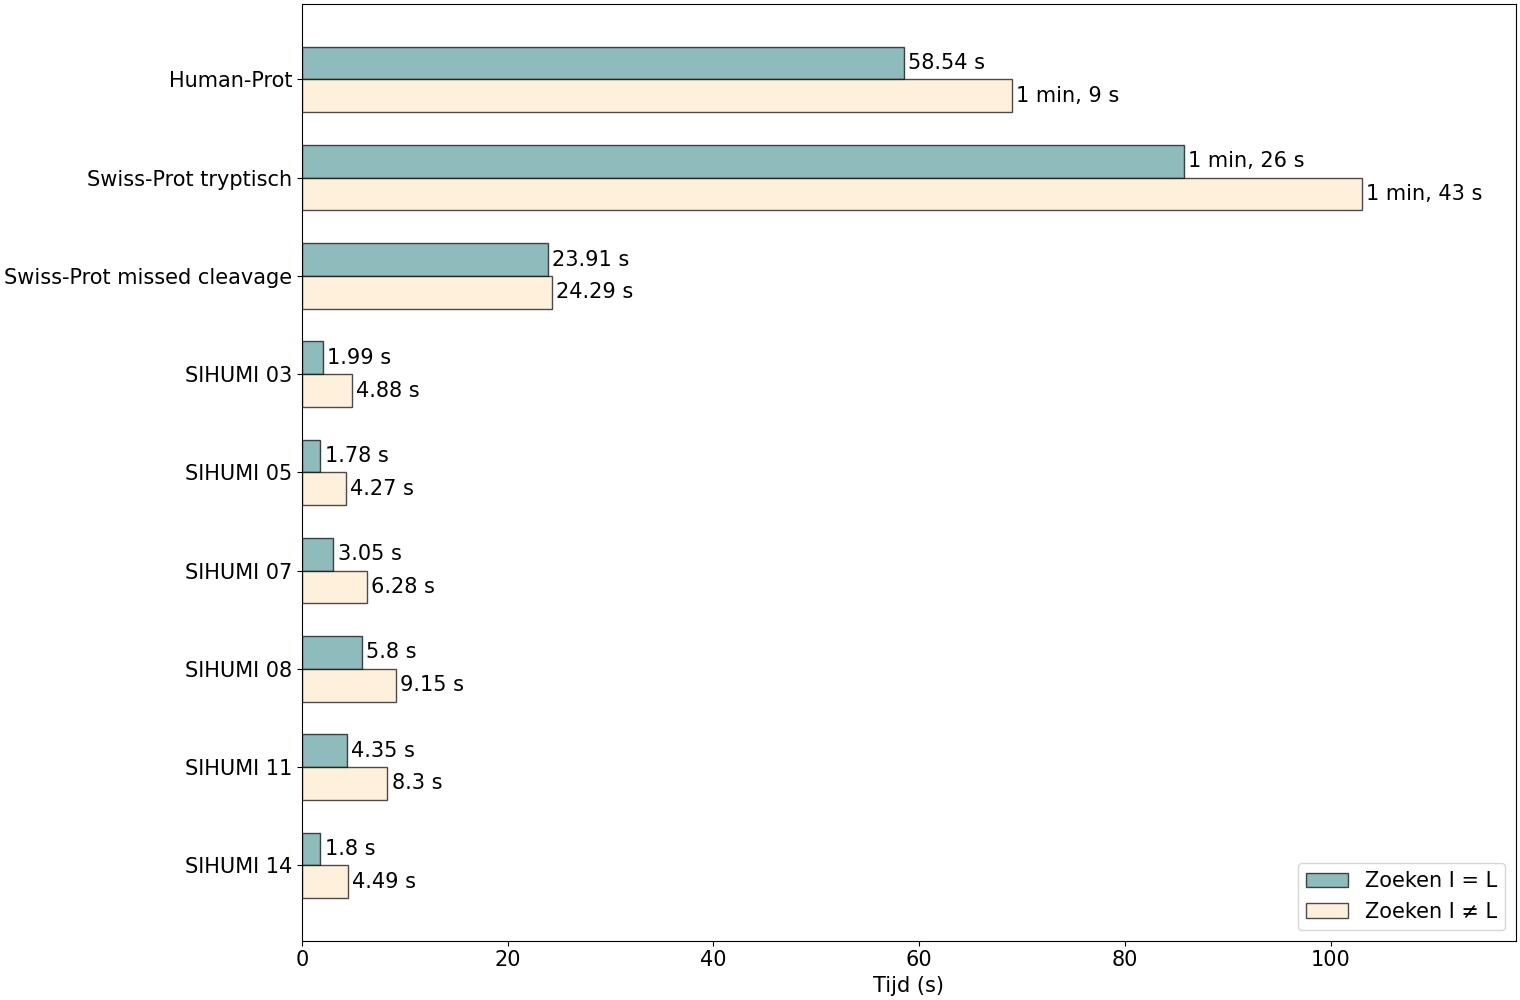
\includegraphics[width=0.95\linewidth]{uniprot_searchtime_standard_vs_il_equality}
    \caption{Zoektijd in UniProtKB (Swiss-Prot + TrEMBL) met en zonder het gelijkstellen van I en L met een SA met sparseness factor $k = 3$.}
    \label{fig:uniprot_search}
\end{figure}

\subsection{Index waarbij I = L}
% TODO

\section{Vergelijking met andere tools}\label{subsec:vergelijking-met-andere-tools}
Aangezien we er in geslaagd zijn om UniProtKB volledig te indexeren is het nuttig om de performantie te vergelijken met bestaande tools.
De tools die we bekijken zijn de \textbf{Uniprot Peptide search tool}, de \textbf{Expasy ScanProsite tool} en \textbf{Unipept} (met de bestaande indexstructuur).
Vanwege de performantie zullen we ons beperken tot het opzoeken van één willekeurige peptide \texttt{ISPAVLFVIVILAVLFFISGLLHLLVR}.
Als referentie gebruiken we de zoektijd in de nieuwe indexstructuur gebruikmakende van een suffix array met sparseness factor 3.
Hierin duurt het zoeken van de peptide \textbf{0.01 seconden} en levert 50 matches op.
Wanneer we I en L gelijkstellen duurt dit opnieuw 0.01 seconden, maar levert dit wel 52 matches op.
Hierbij wordt natuurlijk geen extra tijd geïntroduceerd door een API call over het internet aangezien deze index (nog) niet publiek beschikbaar is.

\subsection{UniProt peptide search tool}
De UniProt peptide search tool\cite{uniprot_search_paper, uniprot_search_site} is een onderdeel van de UniProt site en laat toe om alle voorkomens van een bepaald eiwit te vinden in de volledige UniProtKB database.
Als opties kunnen we kiezen om enkel in Swiss-Prot te zoeken, of in Swiss-Prot en TrEMBL.
Voor beide datasets kunnen we kiezen of we I en L aan elkaar willen gelijkstellen.
Deze features komen exact overeen met de eigenschappen van onze nieuwe indexstructuur.
Qua performantie is deze tool echter extreem onstabiel.
Zo duurt het zoeken van \texttt{ISPAVLFVIVILAVLFFISGLLHLLVR} in de volledige UniProtKB database \textbf{enkele seconden tot zelfs 20 minuten}.
Bovendien vermoeden we ook dat er een vorm van caching toegepast wordt aangezien het zoeken voor een tweede keer zo goed als onmiddellijk het resultaat geeft.
Dit maakt het benchmarken extreem moeilijk.
Zoals verwacht zijn de gevonden matches identiek aan de matches die onze nieuwe indexstructuur vindt.
Naast de variabele performantie faalt deze tool ook regelmatig tijdens het berekenen en ophalen van de resultaten.

\subsection{Expasy ScanProsite tool}
De Expasy ScanProsite tool\cite{scanprosite} laat toe om aan de hand van een taaltje die lijkt op reguliere expressies allerlei patronen te zoeken.
Hun eigen taal laat toe om onder andere wildcards, karakterklasses, inverse klasses en herhalingen te specificeren.
De flexibiliteit van dit systeem is dus een sterk voordeel.
Een nadeel van deze tool is dat niet de volledige UniProtKB databank doorzocht wordt.
Er wordt enkel rekening gehouden met proteïnes die deel uit maken van een reference proteome\footnote{Deze zogenaamde reference proteomes zijn een collectie van eiwitten die door een bepaald organisme gemaakt kunnen worden, en die bovendien taxonomisch belangrijk bevonden worden. Deze laatste voorwaarde wil dus zeggen dat dit niet zomaar van elk organisme is, enkel van een selecte groep organismes die op basis van verschillende factoren belangrijk bevonden wordt. Een voorbeeld hiervan is de \textit{human reference proteome}. Dit zijn alle eiwitten die door een mens aangemaakt kunnen worden.}.
Dit komt er op neer dat ze bij UniProt 2024\_01 \textbf{slechts rekening houden met 85\thinspace152\thinspace388 van de 249\thinspace751\thinspace891 proteïnes}.
Wanneer we de zoekperformantie hier testen duurt het zoeken van de ene peptide zo'n \textbf{5.5 minuten} zonder gelijkstellen van I en L en 15 minuten met het gelijkstellen van I en L\@.
Hierbij zijn er slechts 30 resp. 32 matches gevonden, wegens de subset van proteïnes die gebruikt wordt.

\subsection{Huidige Unipept index}
De bestaande Unipept index laat toe om, \textbf{op voorwaarde dat je peptide tryptisch is}, alle matches te vinden met de keuze om I en L gelijk te stellen.
De peptide die we hier gebruiken is dit ook net, dus zou deze index hiervoor dezelfde matches moeten vinden.
Dit is inderdaad het geval, en gebeurt bovendien gebruikmakende van een API call in \textbf{0.1 seconden}, wat duidelijk extreem veel sneller is dan de andere bestaande opties.
Opnieuw is de zoektijd hier al zo klein dat de invloed van het gelijkstellen van I en L niet te meten valt.
Dat dit enkel werkt voor tryptische peptiden is een extreem grote beperking, volgend voorbeeld illustreert dit.
Stel dat we nu de peptide \texttt{ILAKLFIS} zoeken.
Dit is geen tryptische peptide en bijgevolg kunnen er geen matches gevonden worden.
De nieuwe indexstructuur vindt echter 14 matches zonder I en L gelijk te stellen, en 207 matches bij het gelijkstellen van I en L.


\section{Functionele analyse}
% TODO

\section{Aanbieden van de nieuwe indexstructuur}\label{sec:aanbieden-van-de-nieuwe-indexstructuur}
Alle eerder vermelde benchmarks tonen enkel de zoektijd.
Bij het opstarten moeten we echter \textbf{eerst de indexstructuur inladen}.
Dit alleen duurt 20 tot 25 minuten.
We willen dit inladen slechts eenmalig doen om dan alle requests onmiddellijk af te kunnen afhandelen.
Dit doen we aan de hand van een simpele webserver aan de hand van de Axum crate\cite{axum}.
Deze webserver laadt bij het opstarten de indexstructuur in en blijft daarna wachten op HTTP requests die een JSON bevatten met daarin de peptiden die we willen zoeken.
Op deze manier is dit probleem elegant opgelost, en kunnen we bovendien aan de hand van JSON bestanden erg makkelijk de input verwerken, en de resultaten terugsturen.

